\documentclass{standalone}

\usepackage{tikz}
\usepackage{pgfplots}

% You may be able to remove this if causing issues
\pgfplotsset{compat=1.11}

\begin{document}

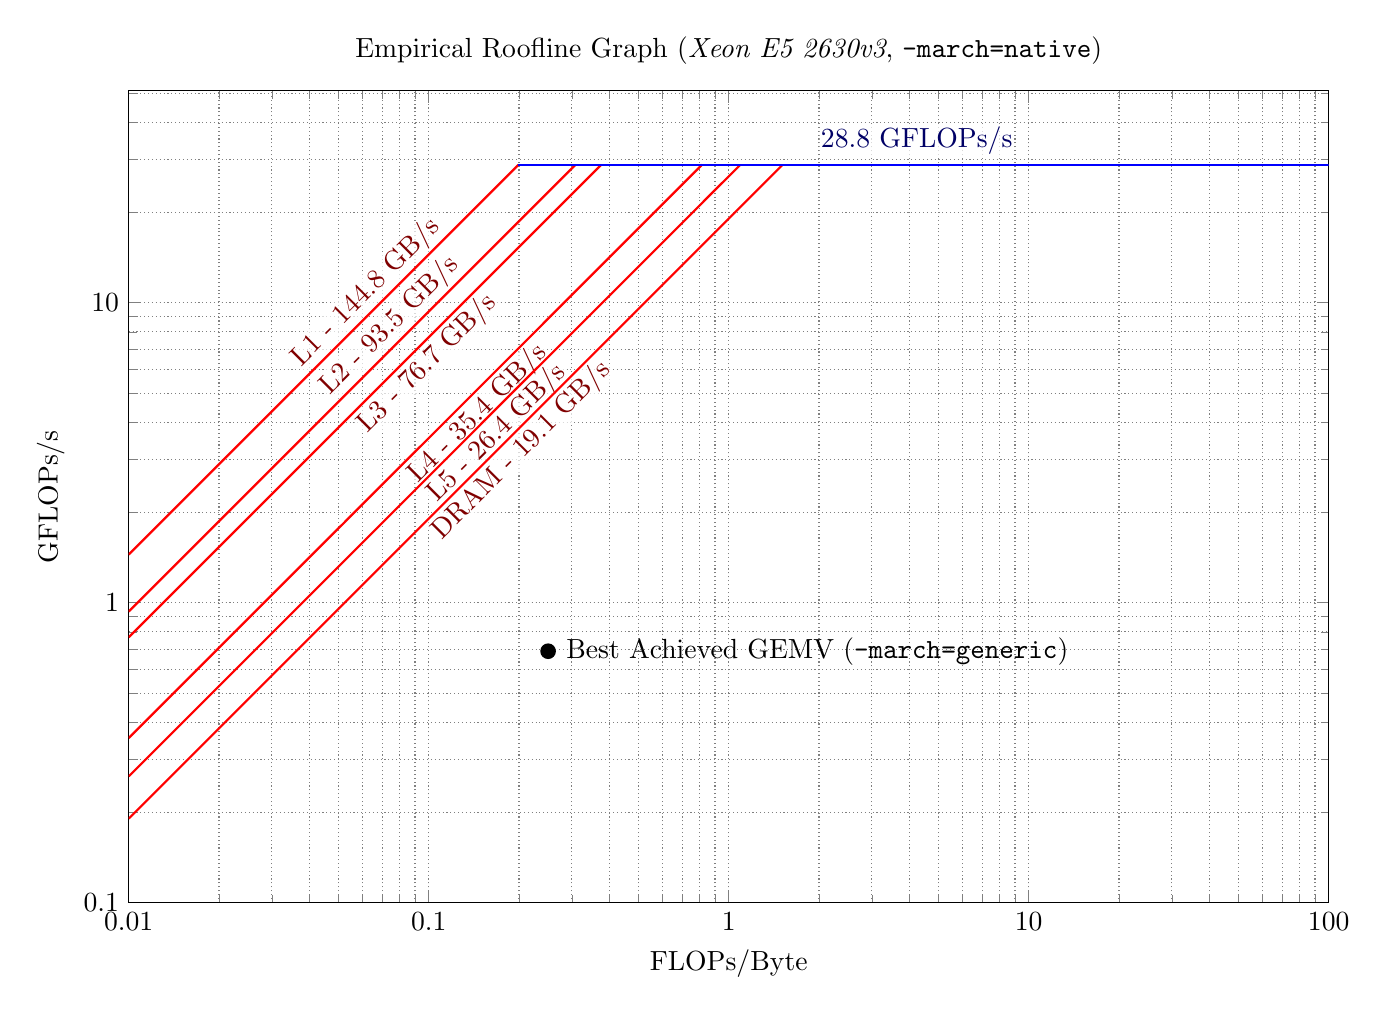
\begin{tikzpicture}
  \pgfplotsset {
    scale only axis,
    axis equal image,
    width=6in,
    /pgf/number format/1000 sep={},
    /tikz/maxline/.style={blue, thick, no marks},
    /tikz/memline/.style={red, thick, no marks},
    /tikz/maxlabel/.style={blue!40!black, right, fill=white, fill opacity=0.7, text opacity=1.0, rounded corners=2pt, inner sep=0.5pt},
    /tikz/memlabel/.style={red!50!black, rotate=45, right, fill=white, fill opacity=0.7, text opacity=1.0, rounded corners=2pt, inner sep=0.5pt}
  }

  \def\Xmin{1.000000e-02}
  \def\Xmax{1.000000e+02}

  \begin{loglogaxis}[
    title={Empirical Roofline Graph (\textit{Xeon E5 2630v3}, \texttt{-march=native})},
    grid=both,
    grid style={black!50, densely dotted},
    xlabel= FLOPs/Byte,
    ylabel= GFLOPs/s,
    xmin=\Xmin,
    xmax=\Xmax,
    ymin=1.000000e-01,
    ymax= ,
    log ticks with fixed point
    ]

    \node[maxlabel] at (axis cs: 2.0000000e+00,3.4608000e+01) {28.8 GFLOPs/s};
    \node[memlabel] at (axis cs: 3.5767736e-02,6.2676591e+00) {L1 - 144.8 GB/s};
    \node[memlabel] at (axis cs: 4.4511958e-02,5.0363990e+00) {L2 - 93.5 GB/s};
    \node[memlabel] at (axis cs: 5.9461629e-02,3.7701621e+00) {L3 - 76.7 GB/s};
    \node[memlabel] at (axis cs: 8.7548925e-02,2.5606252e+00) {L4 - 35.4 GB/s};
    \node[memlabel] at (axis cs: 1.0140368e-01,2.2107678e+00) {L5 - 26.4 GB/s};
    \node[memlabel] at (axis cs: 1.0515176e-01,1.6572265e+00) {DRAM - 19.1 GB/s};

    \addplot[memline, domain=(\Xmin:1.9914376e-01)] {1.4482000e+02*x};
    \addplot[memline, domain=(\Xmin:3.0841621e-01)] {9.3510000e+01*x};
    \addplot[memline, domain=(\Xmin:3.7591241e-01)] {7.6720000e+01*x};
    \addplot[memline, domain=(\Xmin:8.1491947e-01)] {3.5390000e+01*x};
    \addplot[memline, domain=(\Xmin:1.0932525e+00)] {2.6380000e+01*x};
    \addplot[memline, domain=(\Xmin:1.5123230e+00)] {1.9070000e+01*x};
    \addplot[maxline, domain=(1.9914376e-01:\Xmax)] {2.8840000e+01};

    \node[label={0:{Best Achieved GEMV (\texttt{-march=generic})}},circle,fill,inner sep=2pt] at (axis cs:0.8/3.2,0.8/1.160198) {};

  \end{loglogaxis}
\end{tikzpicture}

\end{document}
